\documentclass{IEEEtran}
% \documentclass{article}
\usepackage[utf8]{vietnam}
\usepackage{tabularx}
\usepackage{geometry}
\usepackage{longtable}
\usepackage{blindtext}
\usepackage{graphicx}
\usepackage{hyperref}
\usepackage{caption}
\usepackage[sorting=nyt]{biblatex}
\geometry{
  paper=a4paper,
  left=3cm,
  right=2cm,
  vmargin=2cm,
  includeheadfoot=true,
  headheight=30pt
}
\addbibresource{references.bib}
\begin{document}
\title{\large{ \textbf{MỘT KHUÔN KHỔ HỖ TRỢ LỰA CHỌN DỊCH VỤ CỦA CÁC NHÀ CUNG CẤP ĐIỆN TOÁN ĐÁM MÂY DỰA TRÊN ĐIỂM CHUẨN CẤU HÌNH MÁY ẢO}} \\[10pt] 
\normalsize{A SUPPORTING FRAMEWORK FOR SERVICE SELECTION OF CLOUD PROVIDER \\  BY VIRTUAL MACHINE ‘S SPEC BENCHMARK}}
\author{\IEEEauthorblockN{Son Nguyen-Hong\IEEEauthorrefmark{1}} \\
\IEEEauthorblockA{University of Information Technology - Vietnam National University HoChiMinh City \\
sonnh.17@grad.uit.edu.vn}}

\maketitle

% \textbf{TÊN ĐỀ TÀI:MỘT KHUÔN KHỔ HỖ TRỢ LỰA CHỌN DỊCH VỤ CỦA CÁC NHÀ CUNG CẤP ĐIỆN TOÁN ĐÁM MÂY DỰA TRÊN ĐIỂM CHUẨN CẤU HÌNH MÁY ẢO} \\

% \textbf{TÊN ĐỀ TÀI TIẾNG ANH: A SUPPORTING FRAMEWORK FOR SERVICE SELECTION OF CLOUD PROVIDER BY VIRTUAL MACHINE ‘S SPEC BENCHMARK} \\

\textbf{TÓM TẮT}: Trong giai đoạn phát triển mạnh mẽ của điện toán đám mây, việc lựa chọn dịch vụ và nhà cung cấp phù hợp là một thách thức đáng kể. Số lượng nhà cung cấp rất lớn, mỗi nhà cung cấp lại cung cấp nhiều dịch vụ với mức giá và cam kết chất lượng khác nhau. Những cam kết này phức tạp và thường không dễ kiểm chứng, vì công cụ theo dõi hiệu suất thường được thiết kế bởi từng nhà cung cấp. Do đó, việc lựa chọn đòi hỏi sự hiểu biết cao về lĩnh vực này hoặc việc thuê những chuyên gia từ nhà cung cấp. Điều này đã làm giảm sự đơn giản và tiết kiệm mà điện toán đám mây mang lại. \\

Từ nhu cầu đó, CloudBench được phát triển như một công cụ hỗ trợ người dùng trong việc lựa chọn dịch vụ từ các nhà cung cấp điện toán đám mây. CloudBench sử dụng terraform API để tự động tạo các máy ảo Linux trên các nền tảng như AWS và GCP. Đồng thời, nó sử dụng các công cụ như Passmark, FIO, Iozone và Speedtest để đo lường hiệu suất của CPU, bộ nhớ, disk và network. Các thông số thu thập từ các máy chủ được hiển thị một cách trực quan thông qua Grafana. Người dùng có thể truy cập vào trang web để xem biểu đồ và bảng thống kê, đánh giá tổng quan, so sánh hiệu năng và giá cả của các nhà cung cấp điện toán đám mây, từ đó đáp ứng được yêu cầu kỹ thuật của họ. \\

\textbf{GIỚI THIỆU}: Khái niệm về điện toán đám mây lần đầu được đưa ra bởi Jonh McCarthy: “Một ngày nào đó máy tính có thể được tổ chức và cung cấp như một tiện ích công cộng như dịch vụ điện thoại hay vận chuyển"\cite{garfinkel1999architects}. Từ đó tới nay, rất nhiều công ty lớn như Amazon, Google, Microsoft đã tham gia vào sân chơi này, tạo ra rất nhiều sản phẩm dịch vụ để đáp ứng nhu cầu ngày càng tăng của thị trường. Song hành với đó, số lượng dịch vụ có thể sử dụng càng ngày càng lớn. Chỉ riêng ba nhà cung cấp lớn nhất là Amazon, Google, Microsoft đã lên tới hơn 600 dịch vụ . Mỗi dịch vụ trong đó lại bao gồm nhiều loại với những sự lựa chọn đa dạng. Một \textit{"ma trận"} các lựa chọn đòi hỏi lượng kiến thức hoặc kinh phí lớn để đi đến quyết định đúng đắn.\\
% Một trong những công ty đầu tiên bắt đầu hiện thực hóa ý tưởng điện toán đám mây là Salesforce. Công ty này cung cấp dịch vụ quản lý quan hệ khách hàng dưới dạng SaaS\footnotemark \footnotetext{Software as a service}.
% \cite{amazon2023whatis,googlecloud2023product,Azure2023WhatisAzure}

\begin{figure}[h!]
  \centering
  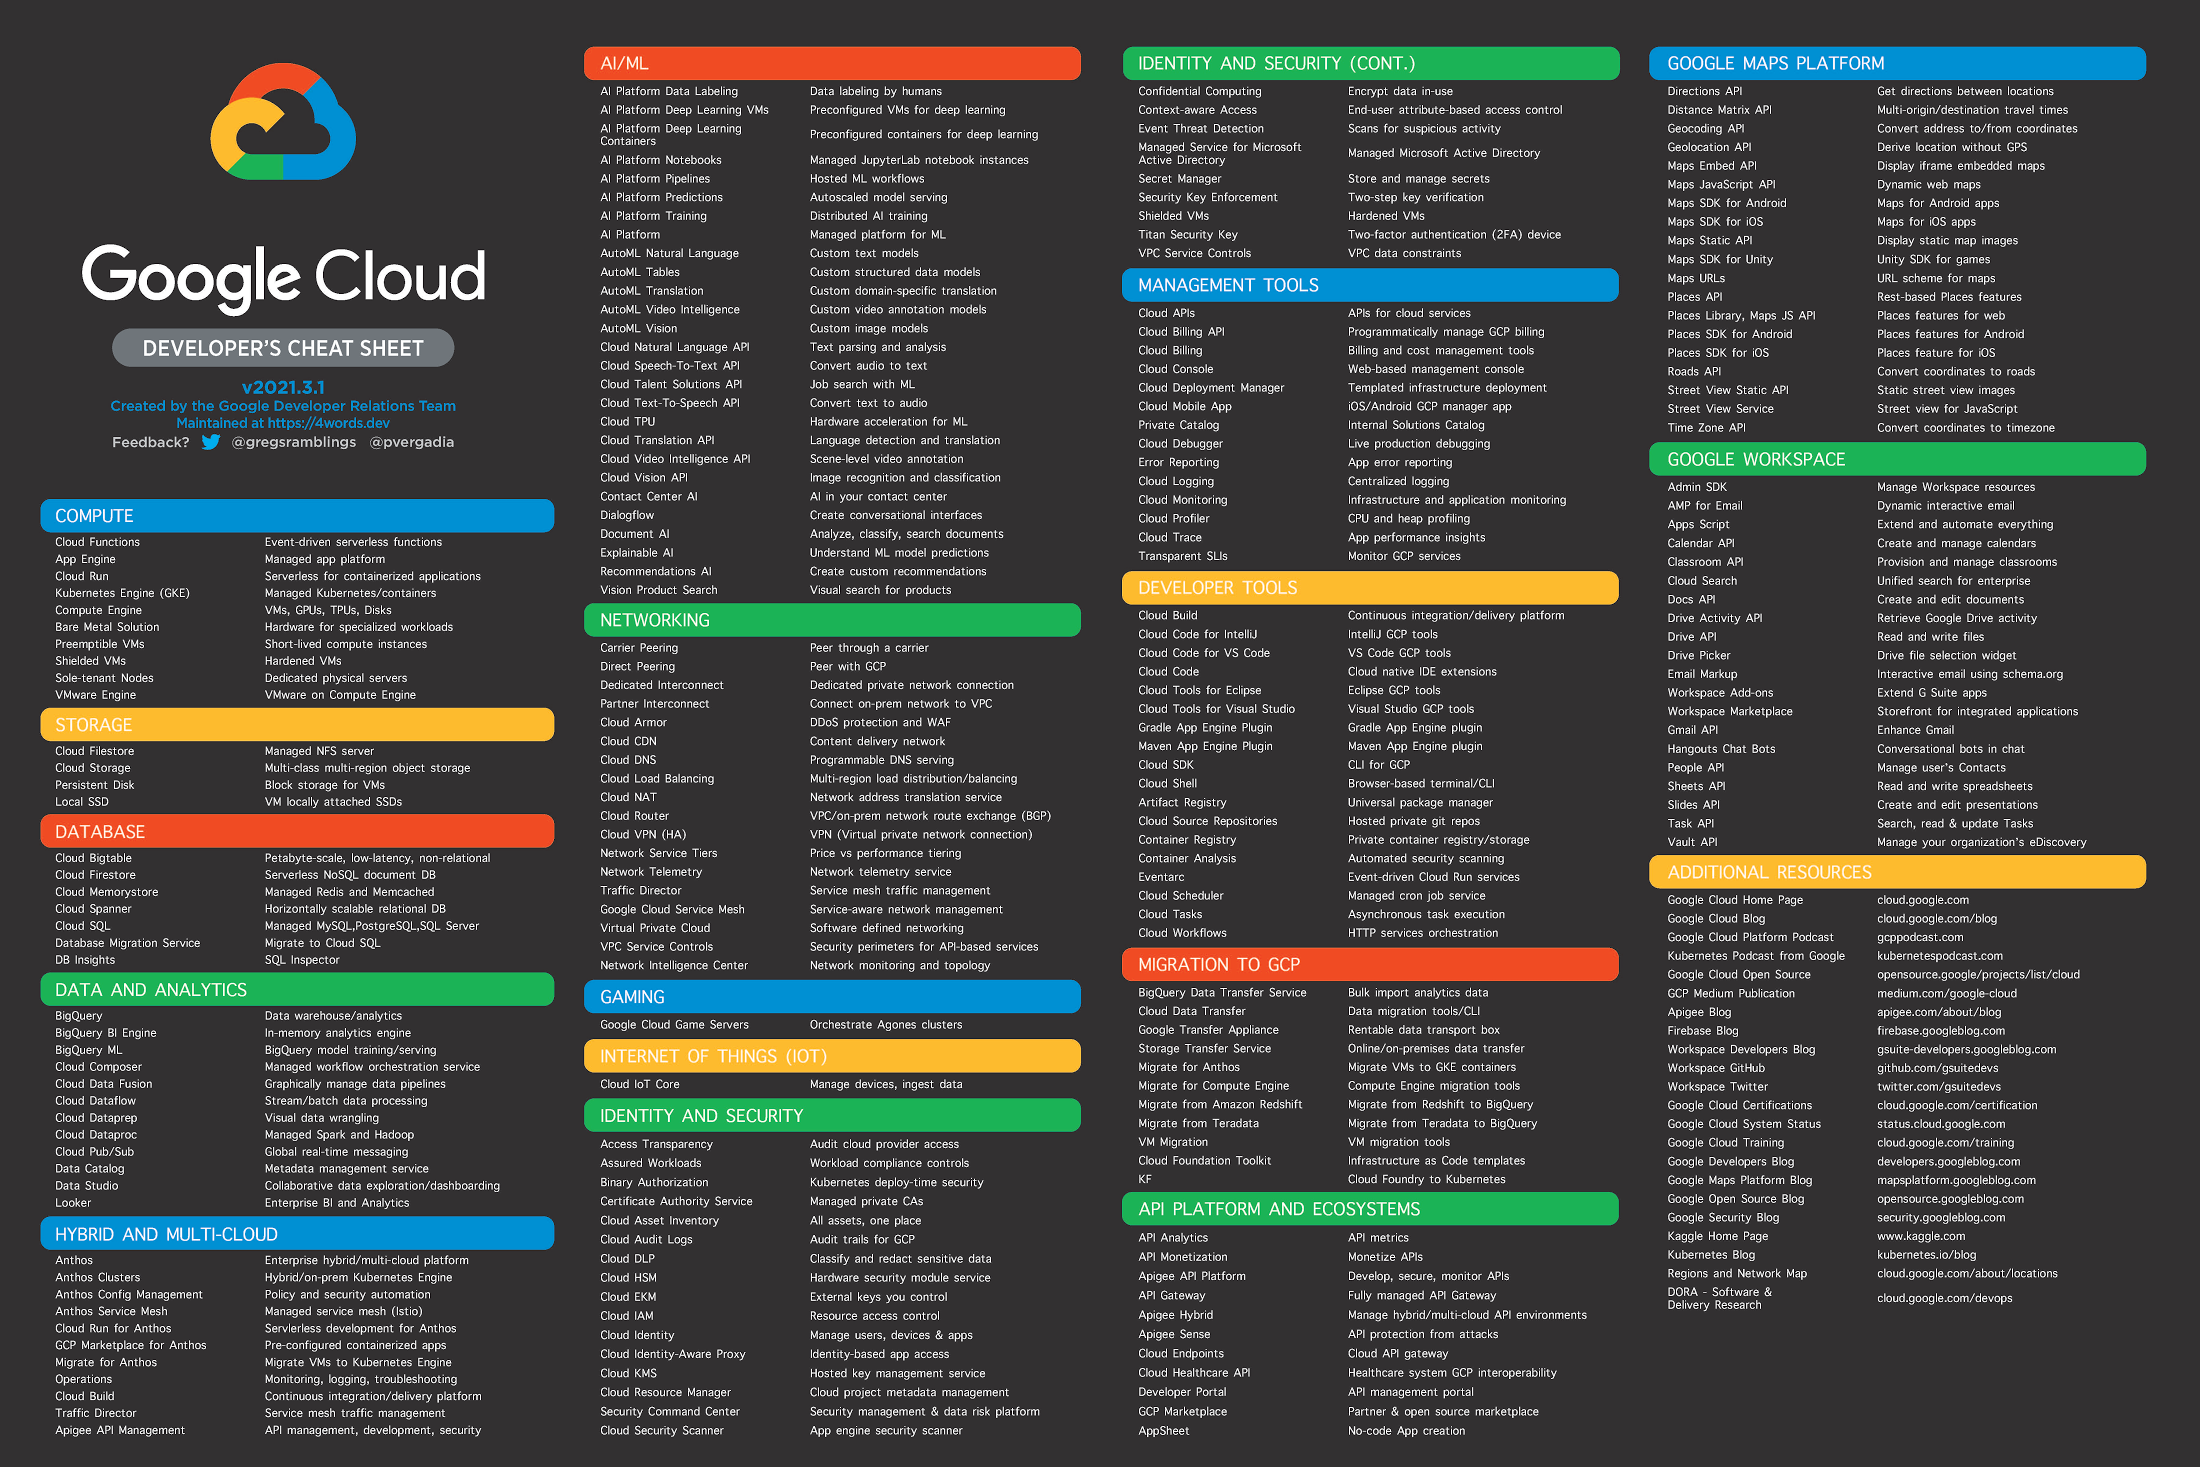
\includegraphics[scale=0.1]{imgs/gcp_services.jpg}
  \caption{GCP services}
  \label{fig:gcp-services}
\end{figure} 
\begin{figure}[h!]
  \centering
  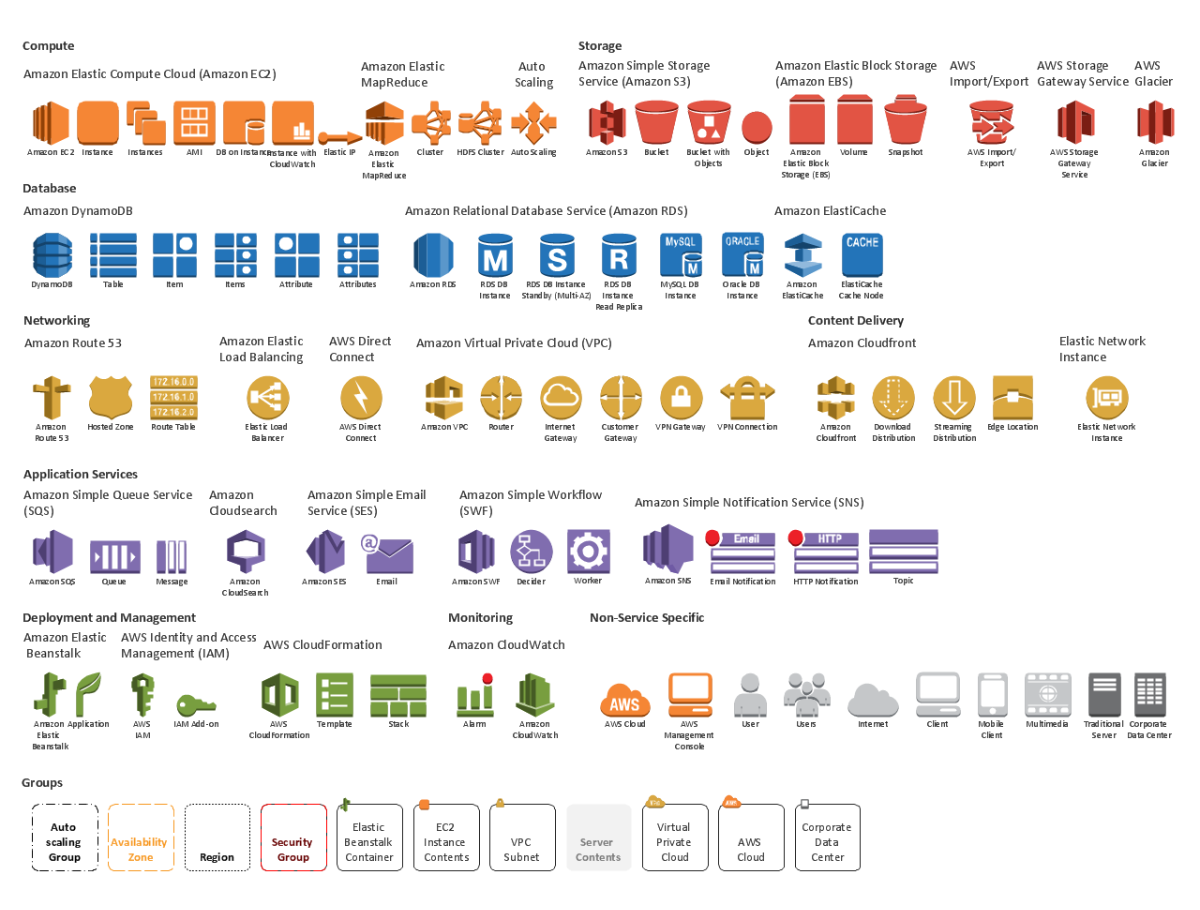
\includegraphics[scale=0.18]{imgs/aws-toolkit.png}
  \caption{AWS Services}
  \label{fig:aws-services}
\end{figure} 

% \begin{figure}[!htb]
%   \begin{minipage}{0.48\textwidth}
%     \centering
%     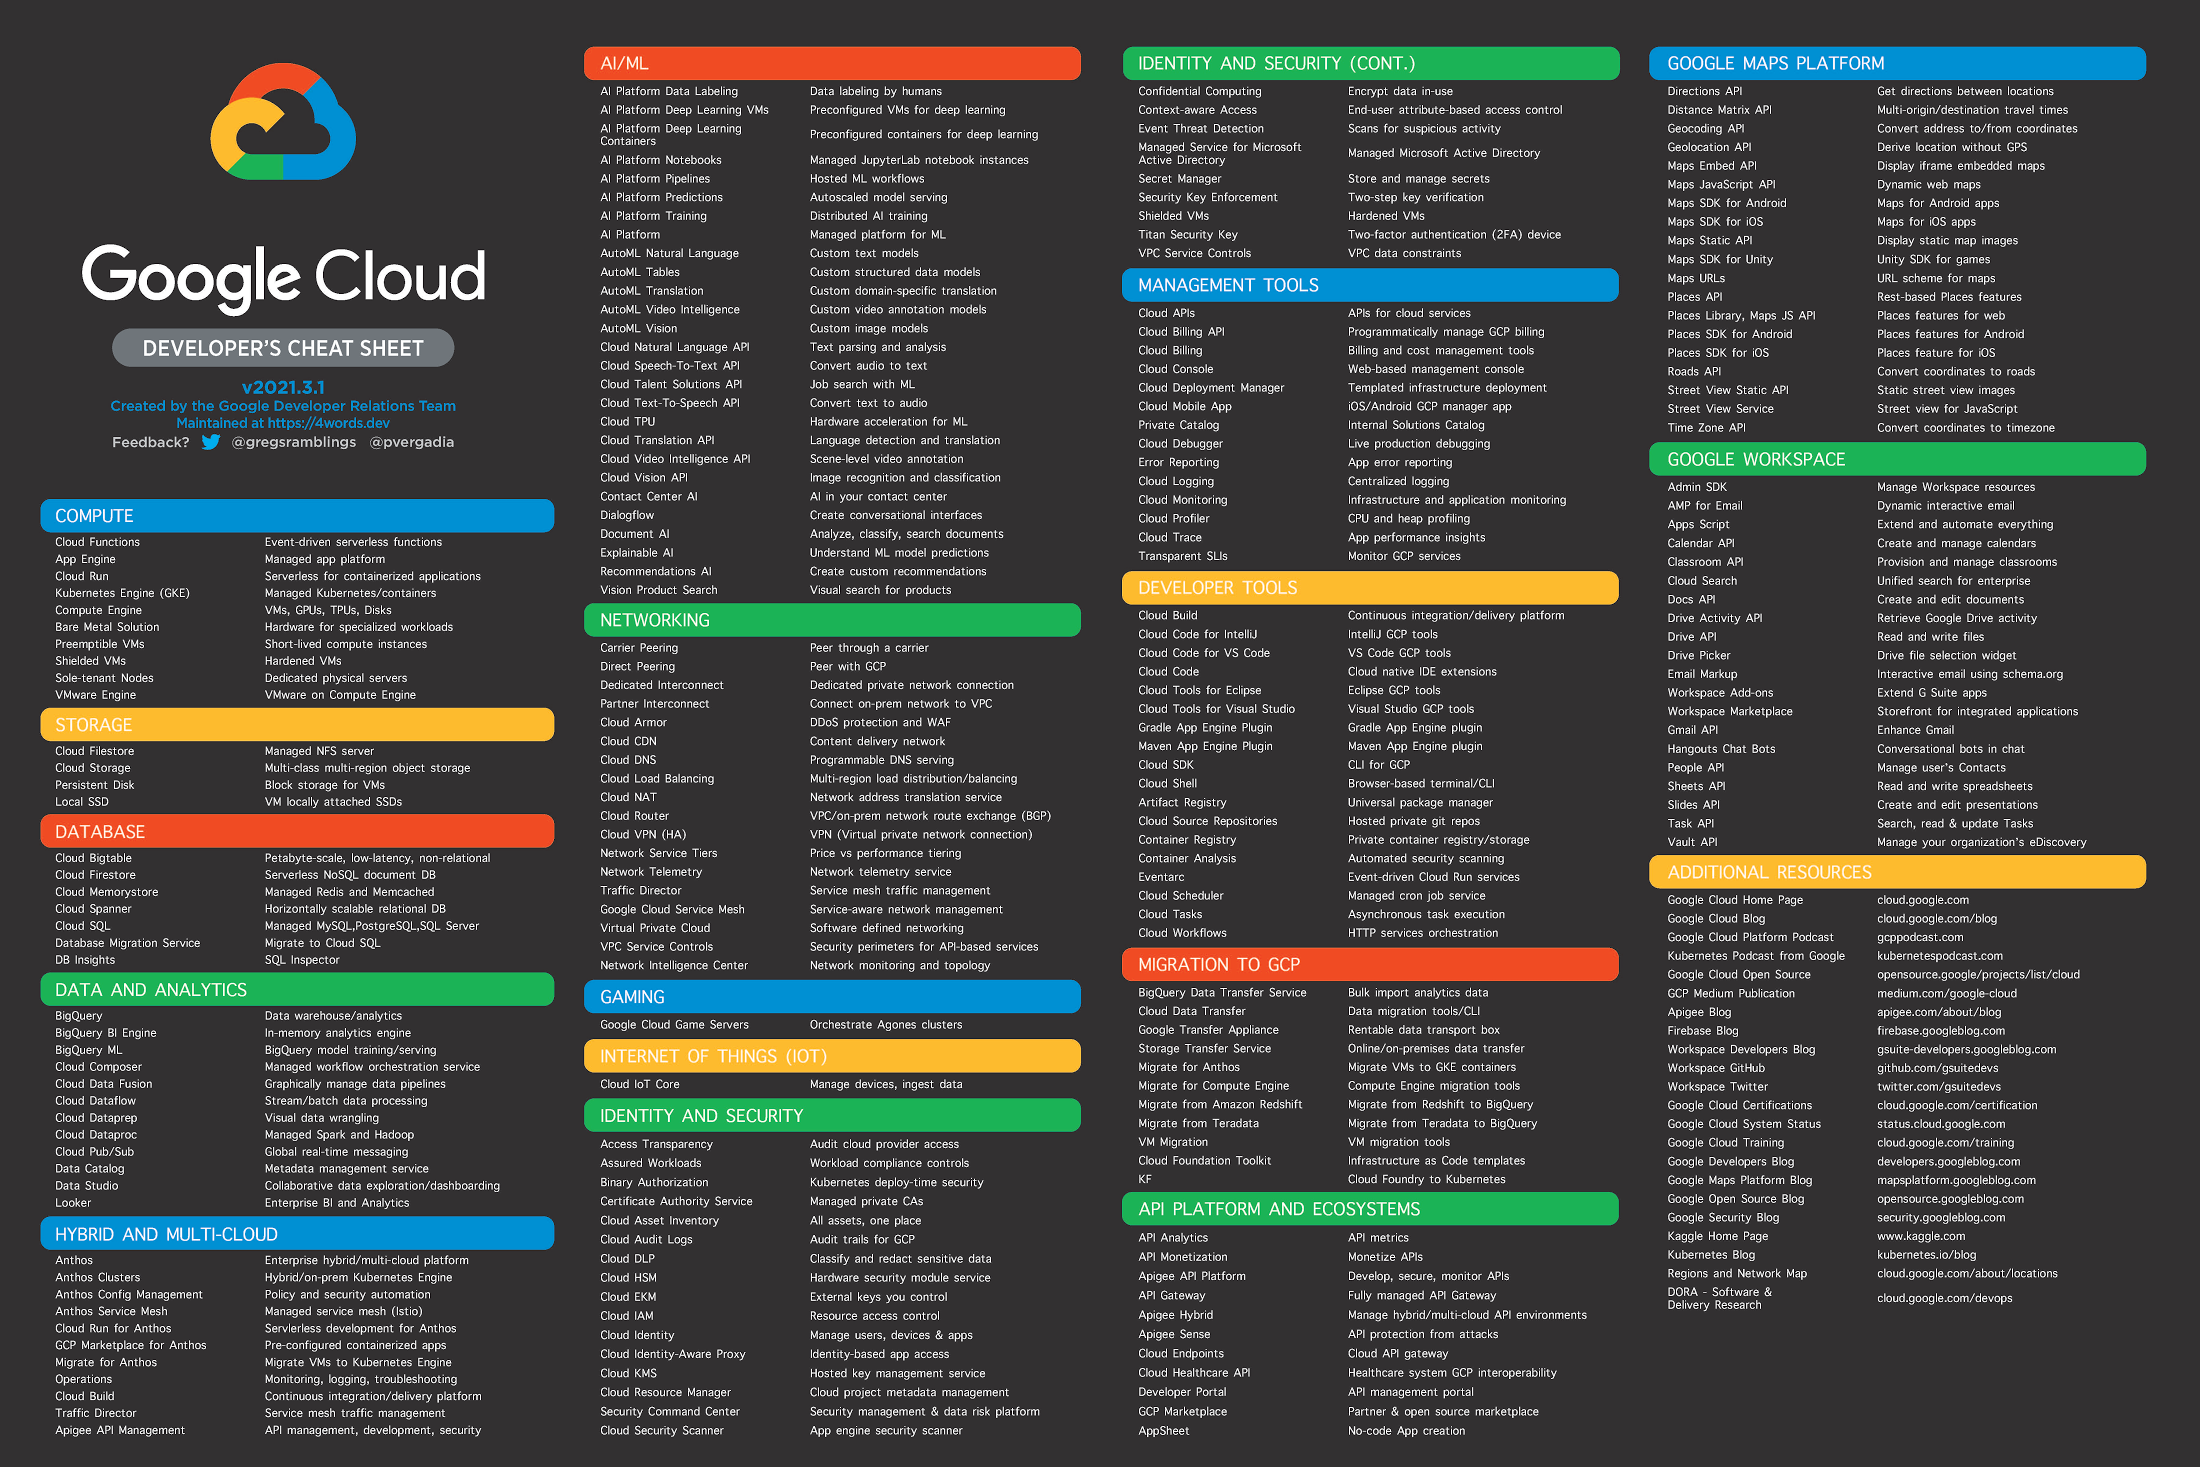
\includegraphics[width=.7\linewidth]{imgs/gcp_services.jpg}
%     \caption{GCP services}\label{Fig:gcp_services}
%   \end{minipage}\hfill
%   \begin{minipage}{0.48\textwidth}
%     \centering
%     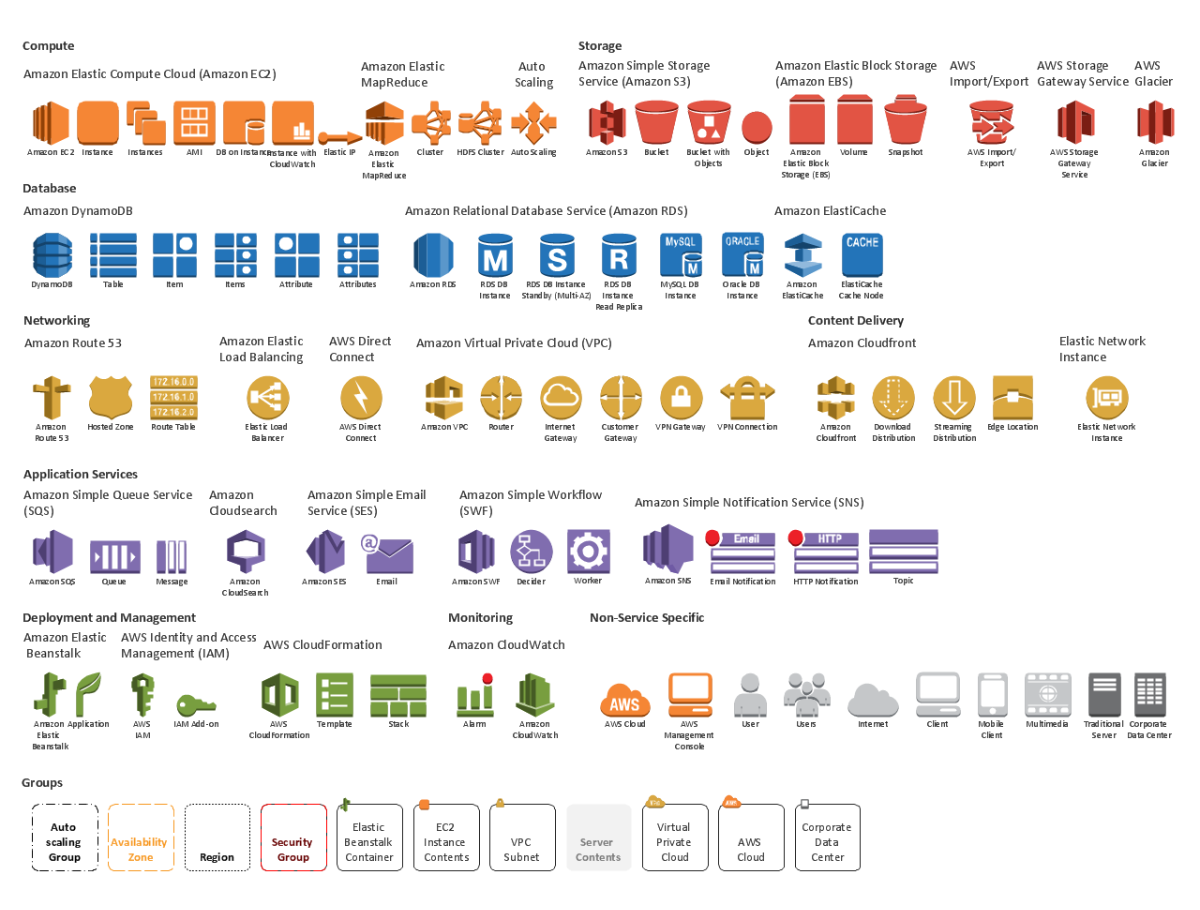
\includegraphics[width=.7\linewidth]{imgs/aws-toolkit.png}
%     \caption{AWS Services}\label{Fig:aws_services}
%   \end{minipage}
% \end{figure}

Hiểu được những yêu cầu đó, các nhà cung cấp có những xuất bản riêng \cite{geewax2018google, wittig2018amazon} giúp người dùng dễ dàng hơn trong lựa chọn dịch vụ. Tuy vậy, những xuất bản này có những hạn chế như được thiết kế quá dài, quá chi tiết tới những cam kết, tính năng, những nội dung tổng quan còn chưa đầy đủ. Cơ cấu tính giá dịch vụ chưa thực sự rõ ràng bởi có quá nhiều hạng mục được tính phí. Một hạn chế khác là các xuất bản này, do hạn chế về luật và quy tắc kinh doanh, chưa đưa ra được những đánh giá về dịch vụ của mình và các đối thủ cạnh tranh trực tiếp. \\

Trong đề tài này, chúng tôi nghiên cứu các công cụ đã được kiểm chứng\cite*{Passmark2023Performancetest, Axboe2023fio, Iozone2016Benchmark, OOKLA2023Speedtest} để tiến hành điểm chuẩn máy ảo Linux của AWS và GCP và áp dụng các phương pháp mới để tự động hóa quá trình điểm chuẩn. Đây là những công cụ mã nguồn mở (hoặc có phiên bản sử dụng miễn phí) manh, cộng đồng lớn và có dữ liệu tham chiếu tốt. Grafana\cite{chakraborty2021grafana} cũng được nghiên cứu như là một ứng dụng để thể hiện các thông số thành biểu đồ, bảng biểu giúp người dùng trực quan so sánh. \\

\textbf{Input:} Thông tin nhà cung cấp \textit{(aws, gcp)} và loại máy chủ ảo \textit{(m5.xlarge, m5.2xlarge, c5.xlarge, c2-standard-4, n1-custom-4-16384)}\\

\textbf{Output:} Một nhóm biểu đồ thể hiện tương quan giữa các loại máy chủ ảo \textit{(như hình \ref{fig:grafana-dashboard})}. \\

\begin{figure}[h!]
  \centering
  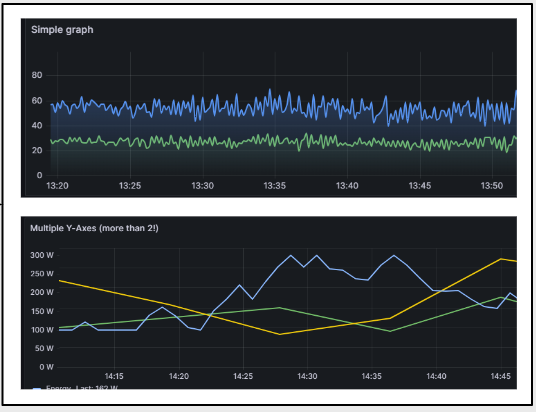
\includegraphics[scale=0.5]{imgs/grafana-dashboard.png}
  \caption{Mô tả kết quả đề tài trên dashboard}
  \label{fig:grafana-dashboard}
\end{figure}
% \begin{figure}[h!]
%   \centering
%   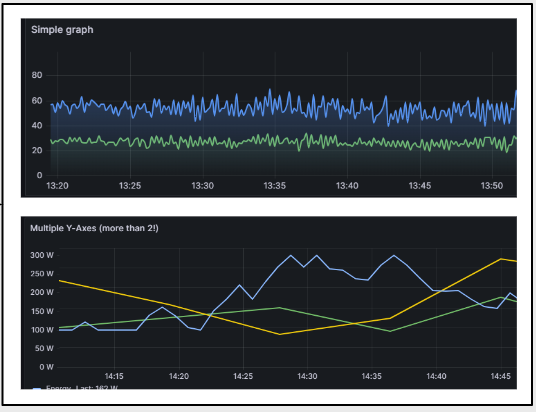
\includegraphics[scale=1.0]{imgs/grafana-dashboard.png}
%   \caption{Mô tả kết quả đề tài trên dashboard}
%   \label{fig:grafana-dashboard}
% \end{figure}
\textbf{Mục tiêu:} Nghiên cứu các phần mềm điểm chuẩn hiện có\cite*{Passmark2023Performancetest, Axboe2023fio, Iozone2016Benchmark, OOKLA2023Speedtest} và áp dụng chúng trong đánh giá chất lượng của máy ảo, xây dựng ứng dụng minh họa là một website. \\

\textbf{Nội dung:}
\begin{itemize}
  \item Nghiên cứu các phần mềm điểm chuẩn\cite*{Passmark2023Performancetest, Axboe2023fio, Iozone2016Benchmark, OOKLA2023Speedtest} chạy được trên máy ảo, hệ điều hành CentOS7 và có thể tùy chỉnh các thông số RAM/CPU/DISK đầu vào.
  \item Xây dựng ứng dụng tạo máy ảo hàng loạt dựa trên Terraform \cite*{zadka2022terraform} có thể tự động thực thi các phần mềm điểm chuẩn, gửi báo cáo số liệu về máy chủ trung tâm.
  \item Xây dựng ứng dụng website có thể tiếp nhận và xử lý số liệu báo cáo, vẽ sơ đồ và bảng biểu chi tiết thể hiện so sánh tương đối rõ ràng.
\end{itemize} 

\textbf{Phương pháp:}
\begin{itemize}
  \item Tìm hiểu các ứng dụng điểm chuẩn\cite{Passmark2023Performancetest, Axboe2023fio, Iozone2016Benchmark, OOKLA2023Speedtest} có thể cài đặt và chạy trên giao diện dòng lệnh (CLI). Tìm hiểu tham số file\_size, record\_size, location\_node phù hợp với tài nguyên có sẵn.
  \item Tìm hiểu cách đánh giá một máy chủ từ những thông số sẵn có bằng thang đo CPU Mark, CPU Compression...
  \item Tìm hiểu cấu trúc và phương pháp tạo tài nguyên trên đám mây bằng Terraform, tập trung vào virtual machine, VPC, security group.
  \item Thu thập và xây dựng bộ dữ liệu điểm chuẩn các dòng máy ảo, lưu trữ tập trung vào database tương thích với Grafana.
  \item Xây dựng chương trình ứng dụng trên nền web cho phép người dùng truy vấn thông tin các điểm chuẩn sẵn có và yêu cầu mới bộ dữ liệu đối với các tài nguyên chưa được điểm chuẩn.
\end{itemize}

\textbf{Kết quả dự kiến:}
\begin{itemize}
  \item Báo cáo các đặc điểm nổi bật của các phần mềm được sử dụng trong bài toán điểm chuẩn. Kết quả thực nghiệm và so sánh với các phần mềm khác.
  \item Tập dữ liệu CloudBench sử dụng cho bài toán.
  \item Chương trình minh họa tương tự trên \href{https://play.grafana.org/d/000000016/1-time-series-graphs?orgId=1}{Grafana demo}
\end{itemize}
% \bibliographystyle{plain} % We choose the "plain" reference style
% \bibliography{references} % Entries are in the refs.bib file
\printbibliography[heading=bibintoc, title = {Tài liệu tham khảo}]
\end{document}

